\chapter{Validation of QSigEx}
\label{qsigex_validation}

Since QSigEx had not been used in many years some modifications were necessary to get the code up and running. 
This software was previously vetted by SNO and the following sections serve as motivation that the software used here reproduces the results of the vetted analysis.

\section{Polynomial Fits}

Discussed in Sections 3 and 4 of Pierre-Luc's thesis~\cite{plthesis} these fits could fit an arbitrary degree polynomial to the electron neutrino survival probability $P_{ee}$. 
Of particular interest are the fits where the conversion probability $P_{ea}$ was fit as an independent polynomial and not assumed to be $1-P_{ee}$. 
The intended goal there was an analysis of oscillation of electron neutrinos to sterile neutrinos, however the same scheme can be used to test for decays.
Refer to~\cite{plthesis} for details, but these fits essentially vary the parameters of the polynomial for $P_{ee}$ and $P_{ea}$ at each step, use these polynomials to reweight the MC data into 4D PDFs (3D for NCD phase) for the fit, and calculate the likelihood that the data matches those PDFs. 

The polynomial fits come in two forms that differ subtly in how the PDFs are rebuilt as the survival probability function changes.
In the first MC events were binned in neutrino energy prior to the minimization process effectively creating a PDF for each neutrino energy bin. 
During the minimization the average of the polynomial over the neutrino energy bins is applied as a weight to that bin and the PDFs from each bin are summed into the PDF for that step.
This method had the advantage of being very fast, though the effect of averaging over the polynomial in the bin is undesirable.
In the second the neutrino energy was not binned, and at each step in the minimization process all the MC data had to be reweighted by the polynomials event-by-event and built into PDFs. 
This method is much slower but produces more accurate PDFs because it does not average over the polynomials.
The binned fit did not perform well in preliminary testing of the lifetime model, and ultimately the unbinned variety will be used for this analysis.
The only downside to this is that the systematic evaluation will take weeks instead of days.

\section{\texorpdfstring{$P_{ee} + P_{ea}$}{Pee+Pea} Validation}

To validate QSigEx, the $P_{ee} + P_{ea}$ fit to SNO 3-phase data described in Section 7.2 of Pierre-Luc's thesis were run again with the update code. The correlation matrix is shown in \Cref{fig:qsigex_pee_pea_fits} with the deviation from the original correlation matrix show in \Cref{fig:qsigex_pee_pea_fits_dev}. The smallness of the deviation in the correlation matrix from the original confirms that the likelihood function is implemented consistently with previous reviews. Since the likelihood function will be unchanged and only the polynomials will be replaced with the lifetime model predictions, this presumably only leaves the implementation and testing of the lifetime model and resulting fit performance as a review requirement for this analysis. 

\begin{figure}
\centering
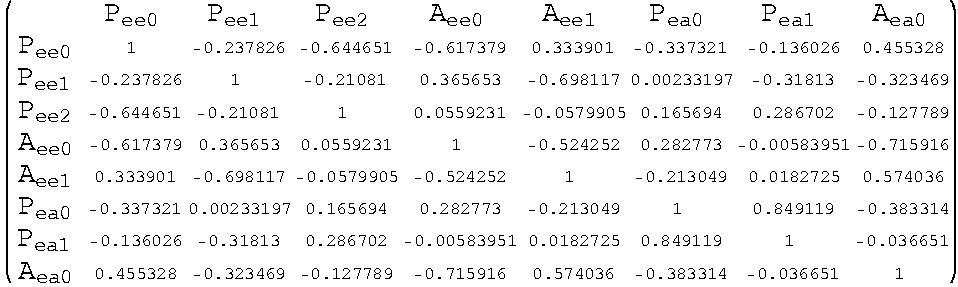
\includegraphics[width=\columnwidth]{corrmat} \\
\caption{
Shown here is the correlation matrix of the fitted parameters for a $P_{ee} + P_{ea}$ fit configured identically to that reported in Section 7 of Pierre-Luc's thesis~\cite{plthesis} to be compared to Table 7.3 in that thesis. The deviation between this matrix and that in Pierre-Luc's thesis is shown in \Cref{fig:qsigex_pee_pea_fits_dev}.
}
\label{fig:qsigex_pee_pea_fits}
\end{figure}

\begin{figure}
\centering
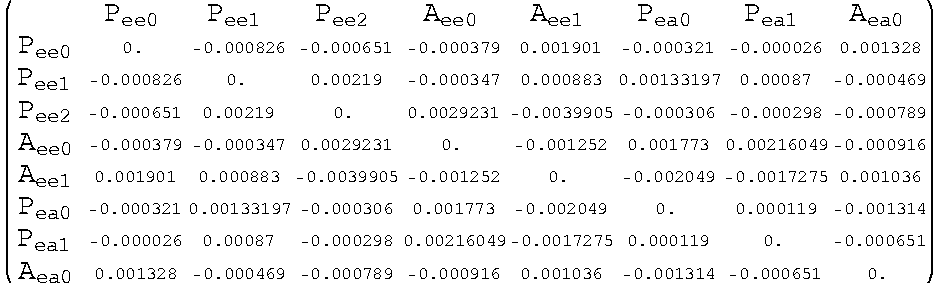
\includegraphics[width=\columnwidth]{dev_corrmat} \\
\caption{
Shown here is the deviation in the correlation matricies of the fitted parameters for a $P_{ee} + P_{ea}$ fit configured identically to that reported in Section 7 of Pierre-Luc's thesis~\cite{plthesis}. Shown here is the difference between \Cref{fig:qsigex_pee_pea_fits} and Table 7.3 in~\cite{plthesis}. The smallness of the values in this matrix demonstrates that a modern day fit with QSigEx produces the same results as when it was originally validated.
}
\label{fig:qsigex_pee_pea_fits_dev}
\end{figure}
